%%% Ch.3: Methodology %%%
\chapter{Methodology and Implementation} \label{ch:method}
The problem of measuring the trustworthiness of communicating entities is an
essential aspect of any online system where they interact with each other for
any purpose, be it shopping, content delivery or file sharing. This chapter
follows on a discussion of a proposed endorsement network where physically or
digitally acquainted entities can endorse each other or their presented
information. The model will address several concerns such as the roles and
requirements of participants as endorser and endorsee, why a participant would
play by the rule and what is to stop them from not doing so, threat models,
etc. With a system of smart contracts, PoC design will confer interaction
between entities, aggregation of information and assignment of scores for final
computation. The storage of data both on and off-chain will be discussed.  

\section{Problem Statement}
To be able to rely on the trustworthiness of an entity as presented by any
online systems, the underlying reputation system needs to be robust and as
transparent as possible. The assurance that available information has not been
tampered with and correctness of claimed identity should be provided to sustain
minimal risk of fraud. The immutable, trustless, decentralized and distributed
attribute of blockchain protocol is a recommended solution on a public
permissionless network.

\section{ User stories \& Requirements} \label{ch:UserStories}
Anyone can join the network and become a participant in the endorsement system.
The two notable roles of a user are endorser and endorsee. An endorser can
initiate the transaction by sending an endorsement to the participant they wish
to. The same user can assume both the roles of endorser and endorsee as long as
a set of predefined requirements are met.  \\ 

%figure - System Context Diagram
\begin{figure}
	\centering
	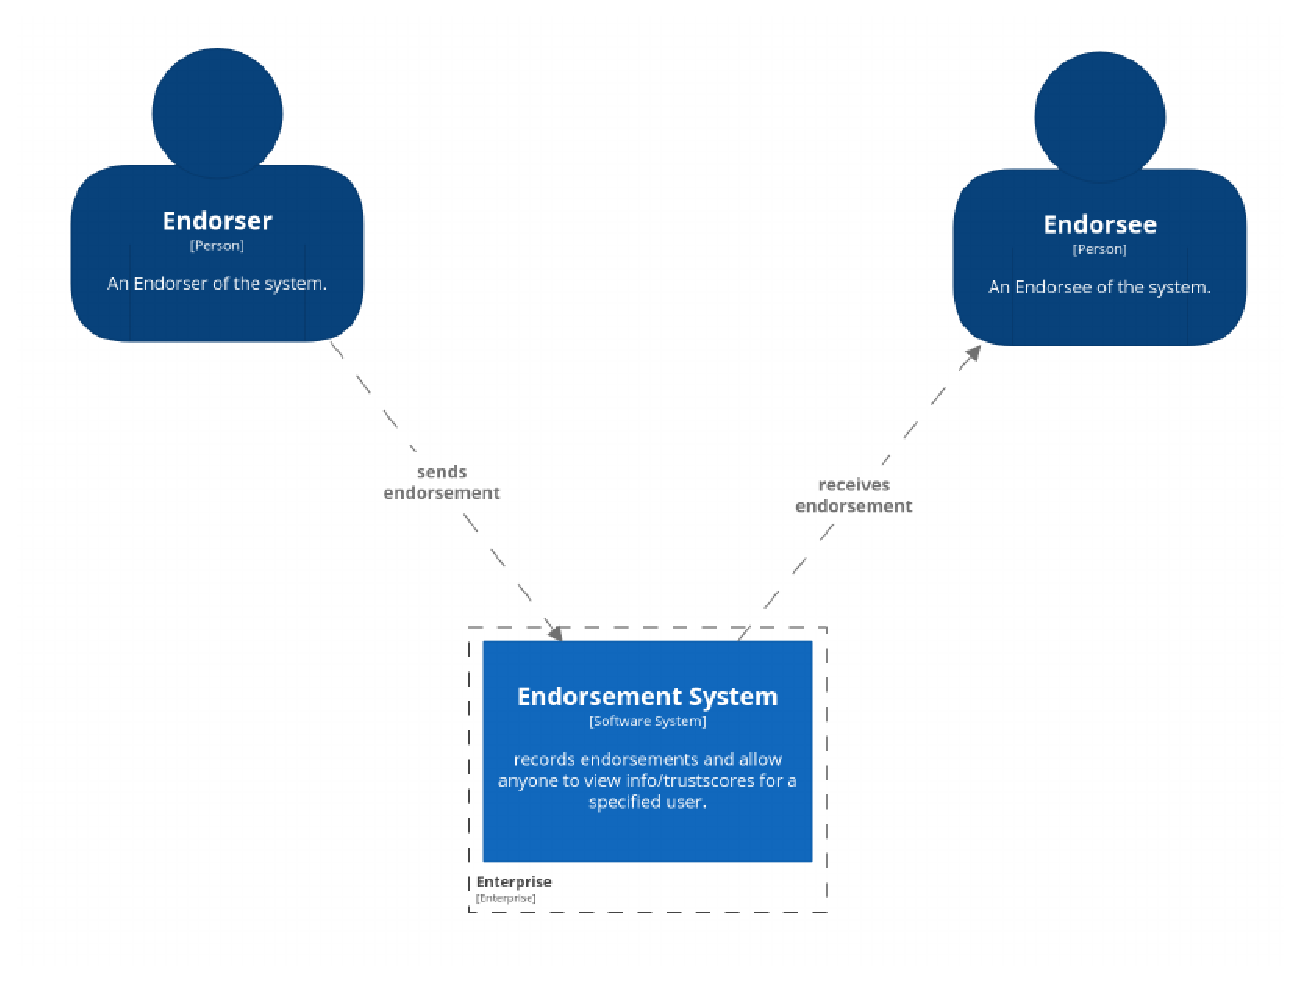
\includegraphics[width=0.9\textwidth]{Images/1SystemContext.eps}
	\caption{Context Layer}
	\label{fig:context}
\end{figure}

The user stories for each role that defines the system requirements for each
user type is presented in table ~\ref{table:userstories}. 
\begin{center} \label{table:userstories} 
	\begin{table}
	\begin{tabular} {| l | p{8cm} | l |}
		\hline
		\textbf{As an}  & \textbf{I need to be able to..}   & \textbf{Traceability} \\
		\hline
		\multirow{2}{*}{Endorser} & send an endorsement so that the endorsement
		is received by the endorsee.& R1
		\\\cline{2-3} 
		& remove endorsement so that the endorsement is removed from the
		endorsee.  & R2 \\\cline{2-3}
		& view a list of endorsees so that i can see to whom i have sent
		endorsements.& R3 \\\cline{2-3}
		& view/edit my personal information so that i can keep it up to
		date& R5 \\\cline{2-3}
		\hline
		\multirow{2}{*}{Endorsee} & view a list of endorsers so that I can see
		from whom I have received endorsements.& R3 \\\cline{2-3}
		\hline
		\multirow{2}{*}{other users} & compute the total endorsement
		impact(i.e., final computed score) of any registered members so that I
		can make an informed decision about the future transactions.
		& R4.1 \\\cline{2-3}
		& make a request to join the endorsement network so that I can start
		sending/receiving endorsements.  
		& R4.2 \\\cline{2-3}
		\hline
	\end{tabular}
	\caption{User Stories and Requirements}
\end{table}
\end{center}

The functional requirements can be listed in points as : \\
\begin{enumerate}
	\item It must be impossible to make an Endorsement if the endorser and
		endorsee is same address or not a registered participant.
	\item It must be impossible to remove an endorsement if the endorser
		doesn't belong to the list of endorsers for the given endorsee.
	\item All the endorsements must be stored such that, it is possible to see: 
		\begin{itemize}
			\item endorser and endorsee for the given endorsement.
			\item degree of incoming and outgoing connections for all endorsers and endorsees.
		\end{itemize}
	\item There must be a way to link the public key hashes to the
		corresponding computed trust scores. 
	\item It must be possible for a participant to edit their own profile if
		the editor is the same as the profile owner. 
\end{enumerate}

The non-functional system requirements are : 
\begin{enumerate}
	\item Security: There should be minimal security considerations taken into
		account while writing the smart contract that can avoid simple bugs.  
	\item Reliability: The data stored on the blockchain should be immutable
		and verifiable by anyone publicly.
	\item Trust metrics should correctly describe the actual trust score/impact of the nodes.  
\end{enumerate}

\section{The Model - Endorsement Network}\label{sec:endorsementModel}
\begin{wrapfigure}{l}{0.5\textwidth}
	\begin{center}
		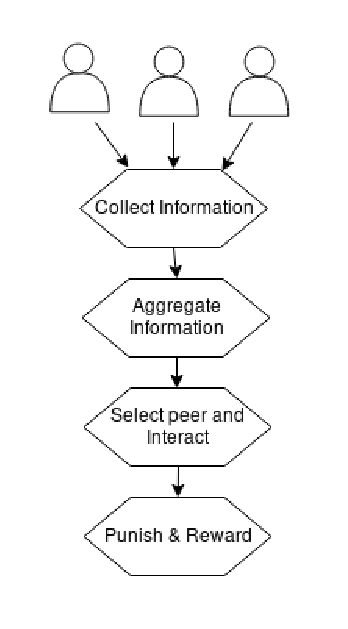
\includegraphics[width=0.2\textwidth]{Images/trustRepSteps.eps}
		\caption{Trust and Reputation Model steps taken from \cite{marmol2009security}}
		\label{fig:truststep}
	\end{center}
\end{wrapfigure}
Complete trust and reputation model consists of four different steps as
depicted in figure ~\ref{fig:truststep}. Among these steps, endorsement network
concentrates on the first two steps, collection, and aggregation of
information. For the last two steps, selecting and interacting with a peer for
transaction based on which they get punished or rewarded is based on a
transactional network. 
As implementing transaction network is not the main task
of this project, feedback based on success or failure of a transaction will be
mostly based on the assumption that can be used by endorsement system.  Thus,
most of the section in this chapter is based on the smart contract logic for
endorsement model and discussion on the possibility to be used by other
transactional systems. 

The initial assumption on endorsement system is that all nodes are honest and
as such receive equal points that they can spend at will once registered on the
network. This received points are the consumable power that keeps depleting
with every endorsement connection made along the way. As can be seen in figure
~\ref{consumablePoint} , these points follow a convergent sequence that
converges to the limit 0 as the number of connection `n' increases. As such,
increasing the number of connection alone will not be enough to achieve a
higher impact on the network.
\begin{figure}
	\centering
	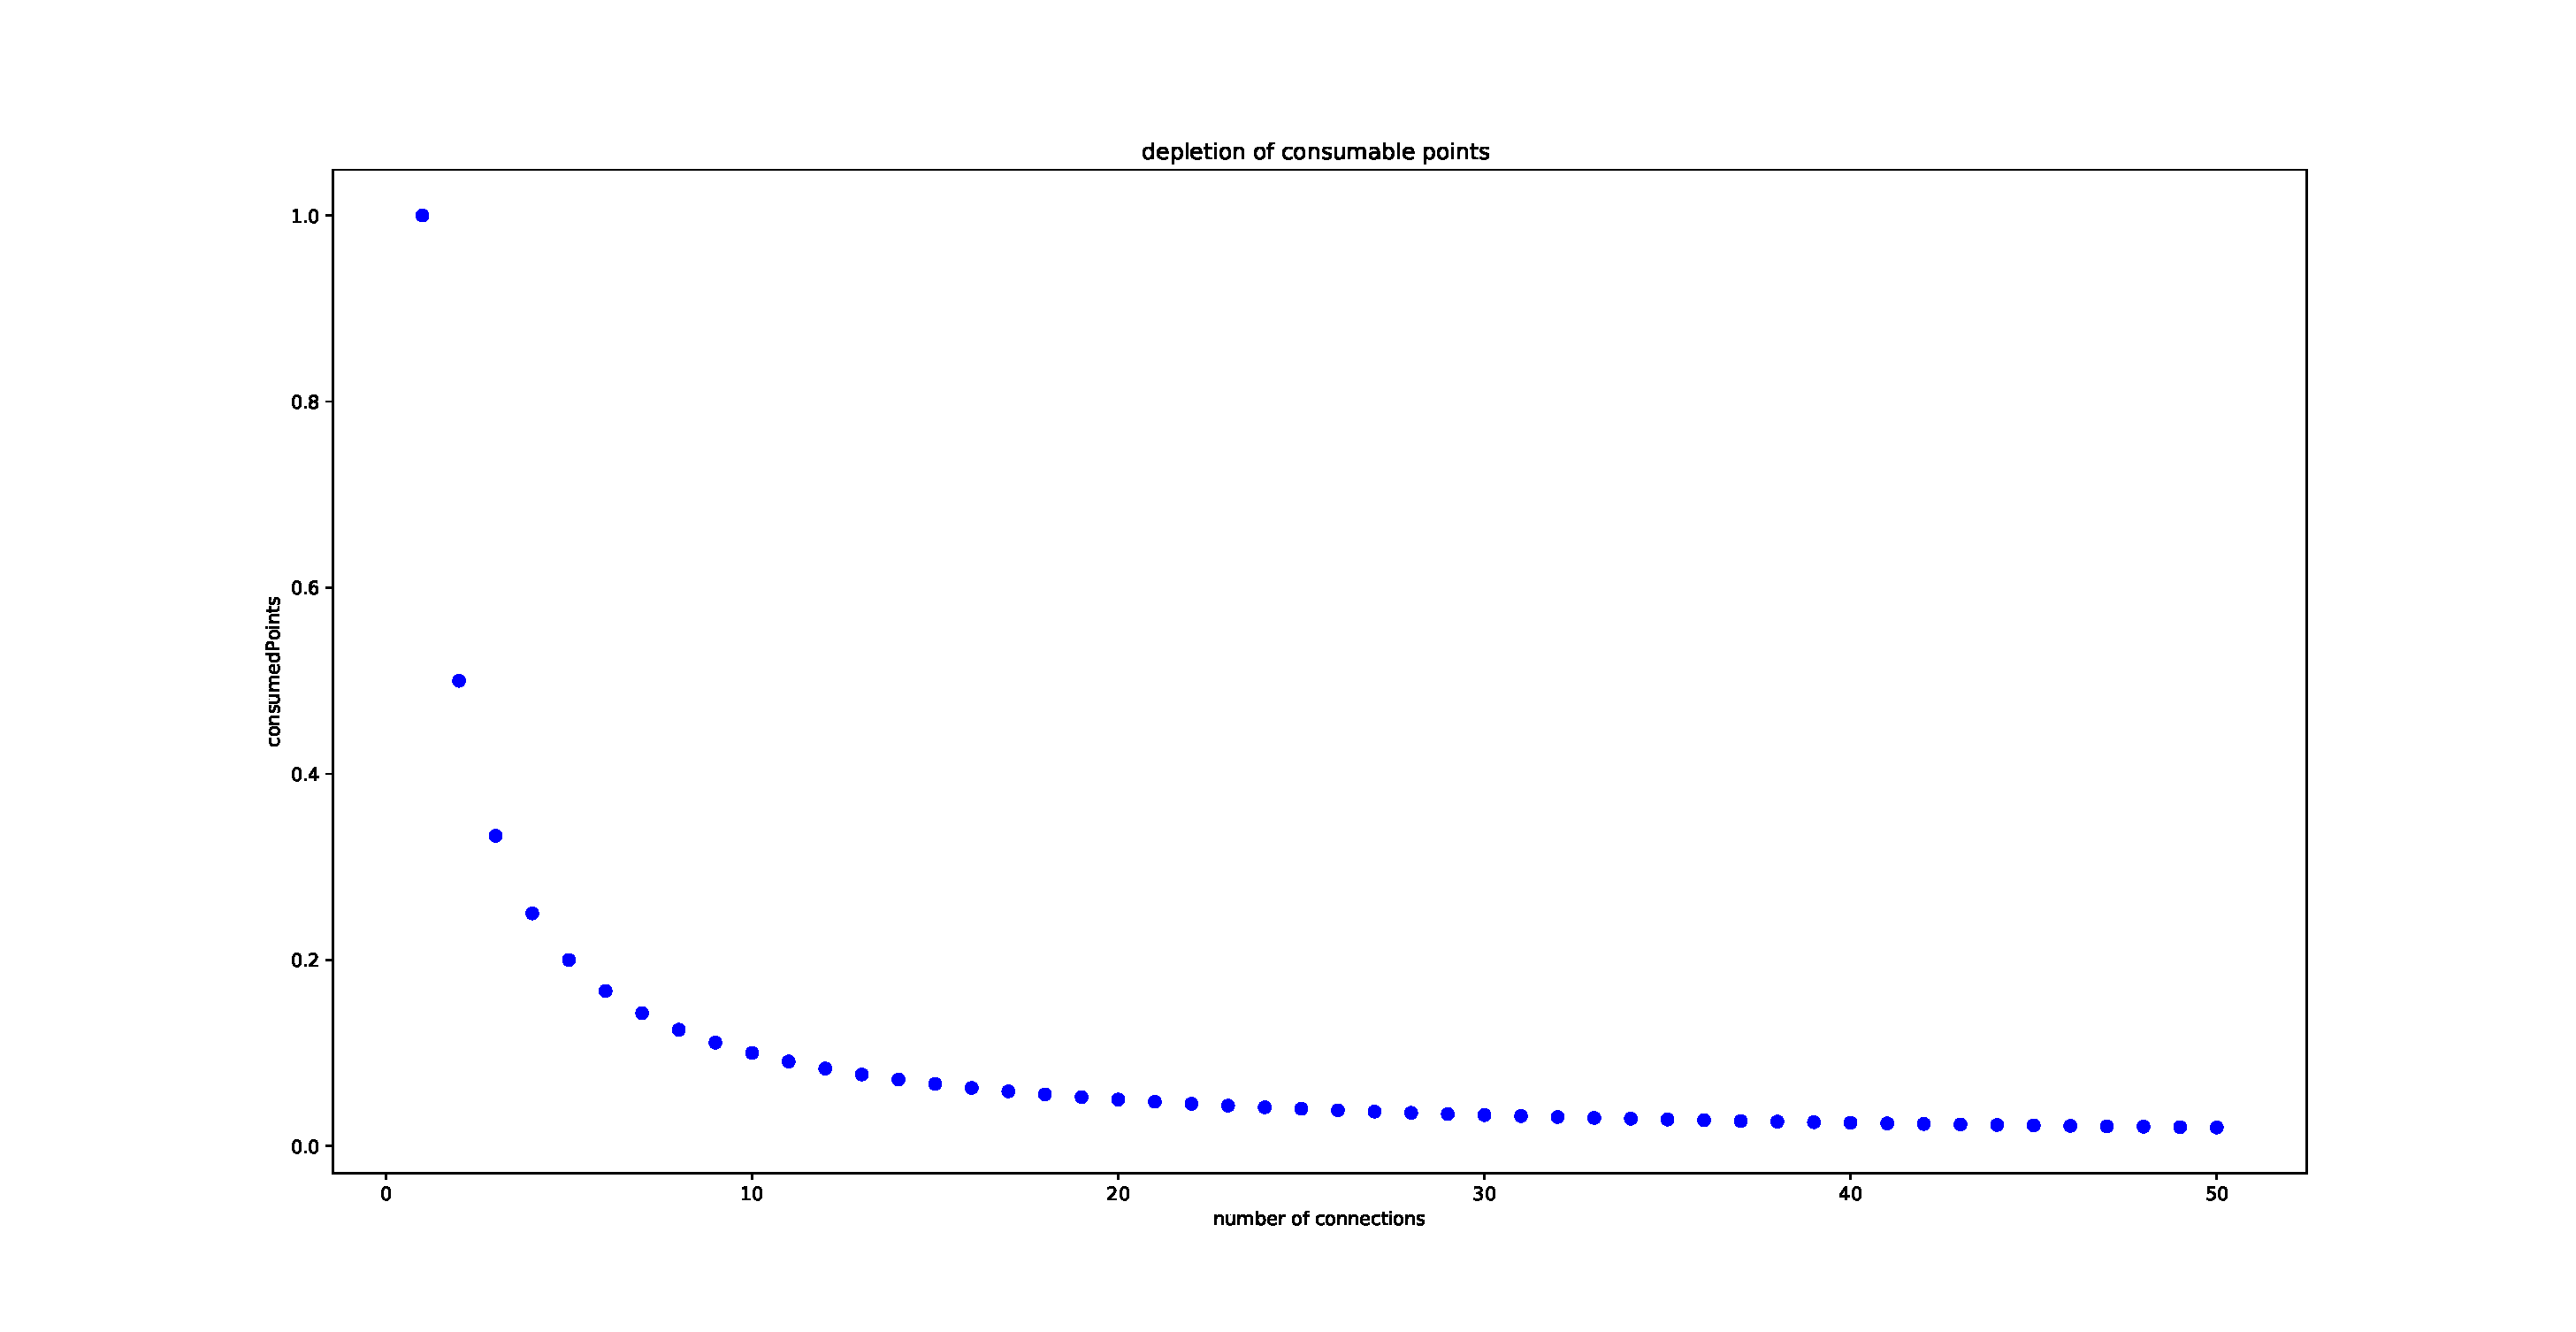
\includegraphics[width=1.0\textwidth]{Images/ConsumablePoints.eps}
	\caption{Convergent behaviour of consumable points as 'n' increases}
	\label{consumablePoint}
\end{figure}

\subsection{Computation of Total Endorsement Impact(TEI)} 
The collection of information refers to the collection of endorsement
interaction between endorsers and endorsees.  Aggregation of them to get the
global trust score, total endorsement impact for all the nodes is made based on
various factors. A short definition of them and the terminology used throughout
the endorsement model is given below. \\ 

\textit{$nEG_A$}: number of endorsements sent by a participant 'A'. \\
\textit{$nER_A$}: number of endorsements received by a participant 'A'. \\
\textit{$ratio_A$}: ratio of \textit{$nEG_A$} to \textit{$nER_A$}. This value
ensures that sent and received endorsement are not far off from  each other.
\textit{$ratio_A$} is always assumed to be less than 1 and is given by: 
\begin{equation}
	ratio_A = \frac{min(nEG_A,nER_A)}{max(nEG_A,nER_A)} 
\end{equation}

\textit{$cp_A$}: Total amounts of points spent by a participant 'A' out of the
initially received consumable points. 1 being the initial consumable points
received by everyone who joins the network, \textit{$cp_A$} is given by
1/\textit{$nEG_A$}.

\textit{$TRP_A$}: This corresponds to A's total received points which is the
accumulated sum of consumed points by all endorser of A.  If a peer 'A'
receives an endorsement from 'n' number of peers, then the \textit{$TRP_A$} is
calculated as:
\begin{equation}
	TRP_A  = \sum_{i=0}^{n}cp_{i}
\end{equation}

Finally, the total endorsement impact made by 'A' is given by: \\
\begin{equation}
	TEI_a = ratio_a * TRP_a
\end{equation}

%
%ratio of nEG and nER to create a balance in the network
%final score considers both given and received, and how much impact endorser of
%an endorsee has made already

\section{Design of PoC}\label{sec:pocDesign}
The PoC design is based on the requirements mentioned in section
\ref{ch:UserStories}. This section explains the design considerations and the
setup of smart contracts used for the EDS system. A high-level overview of the
overall system is presented in figure ~\ref{fig:SystemContainer}. The
visualization is based on an architectural model by \cite{brown2013software}.
It essentially uses three-layer to visualize a software architecture. i.e.,
context layer, container layer, and component layer. The context layer attempts
to describe several user types and their interaction with the system on a high
level. The container layer takes it further by expanding on the software system
and shows a high-level overview of the components involved. The component layer
then goes on to explain in detail the connected component. For endorsement
system, the component that is most relevant and thus explained in detail is the
smart contract.
After the design details, the section ends with the discussion on graph
algorithms that can be used by the transactional network, blockchain
infrastructure, governance model, and storage of information on and off-chain.

\begin{figure}
	\includegraphics[width=0.9\textwidth]{Images/2Container.eps}
	\caption{Container Layer}
	\label{fig:SystemContainer}
\end{figure}

%\subsection{Formalization}
%The endorsement network as a distributed system can be formally defined by : 
%
%\begin{itemize}
%	\item{P: set of participants $\{p_1,p_2,.. ..,p_j\}$ where 'j' is the total
%		number of participants.} 
%	\item{endorse(x,y): x has sent endorsement to y where $x,y \in P$}
%	\item{receive(y,x): y has received endorsement where $x,y \in P$ }
%	\item{Each participant 'p' has a set of endorsers $\{e_1,e_2,.. ..,e_m\}$
%		and a set of endorsees $\{r_1,r_2,.. ..,r_n\}$ if endorse(e,r) and
%		receive(r,e) is true. Here, 'm'is $nEG_p$	and 'n' is $nER_p$.}
%\end{itemize}

\subsection{Design Consideration} \label{subsec:design_considerations}
The design considers possible behavior that can result from the interaction
between nodes, both honest and malicious. The endorsement relation exists based
on a subjective measure from an endorser. Thus, they are known entities based
on physical or digital acquaintance.\\

The acquaintance could be of the following form:
\begin{itemize}
	\item Alice and Bob go to the same school/workplace, have worked on
		multiple projects together and is confident of Bob's reliability.
	\item Alice has dealt many times with Bob in an online shopping website and
		always had an excellent transaction with him. In this interaction,
		Alice is sure that Bob is an honest seller and Bob is confident that
		Alice is a reliable buyer. 
	\item Alice follows Bob on some social media and knows that Bob's
		article is good and sees lots of pre-research in his writing and is
		confident that Bob doesn't engage in the false news.
\end{itemize}
Thus, Alice is likely to endorse Bob and vice-versa on the endorsement network.
They can use secure messaging channels to exchange their keys and endorse each
other. There is no objective way to verify if Alice and Bob are separate entity
sending out an honest evaluation of each other. However, the endorsement
network can receive feedback from the transaction network. Therefore, if any
entity that has received endorsement turns out to be a bad actor in an online
transaction, they can be punished along with the node that sent the
endorsement. i.e., both endorser and endorsee get punished by decreasing the
total endorsement impact by 50\%.
From a game-theoretic perspective of a behavioral outcome, following
definition were made for network influencing factors. 

\begin{enumerate}
	\item \label{item:fakeeds} \textbf{Fake endorsements with pseudonymous
		identities:} Endorsement system being on a
		distributed, public permissionless blockchain network allows anyone to
		join and start sending endorsements immediately to whoever they wish
		to. This creates the possibility that an entity could create multiple
		pseudonymous identities with an aim to inflate their impact on the
		network by increasing nEG or nER for their associated persona.  There
		is no straightforward way to detect and stop this behavior right away.
		However, if doing so doesn't provide any significant advantage, then
		the assumption is that a rational decision would be not to do it.  One
		factor that is believed to stop a participant from making too many
		endorsements is the convergent behavior of consumable points. While,
		there is no limit to the amount of connection a participant can form,
		as the number of connection increases, the value of consumable points
		decreases. 
	\item \textbf{Transaction cost:} Ethereum is a programmable blockchain that
		supports a Turing complete programming language. Thus, to avoid running
		in infinite loops or DDOS attacks, gas was introduced. Every operation
		has a gas cost. One could write a program to do anything they wish to
		do on the network as long as the account that initiates the transaction
		can pay the gas cost of all operations. The gas consumption is an
		imperative aspect of endorsement system for two reasons. \\
		\begin{itemize}
			\item \textit{Standard transactions on Ethereum:} A participant
				that makes a call to 'sendEndorsement' function is responsible
				for paying all the required gas costs. This function updates
				the state variable nEG and nER. While the price may not seem
				too high for making one transaction, a malicious node with
				multiple pseudonymous identities has to pay for all the
				operations initiated by all personas. For instance, given the
				interaction graph in the figure, if Alice is an honest node,
				then she only needs to pay for the operation of one
				transaction. Whereas if both Bob and Charlie are the
				pseudonymous identities of Alice, she needs to pay for six
				transactions. Thus, the assumption is that they may make ether
				transfer at some point between their accounts. This information
				is publicly available for anyone on the ethereum blockchain
				network to view the chain of ownership.  If some interactions
				in the endorsement network look suspicious, one could look up
				this detail. This method is not guaranteed to detect a Sybil
				node on the endorsement network but is just another additional
				factor that might be useful before making a decision. 
			\item \textit{ Local information of all neighbouring nodes:}
				Whenever an endorser makes a new connection, the nEG, and
				consumable point change accordingly. This change in consumable
				point has to be reflected for the list of all endorsees. This
				is not to be confused with a one time update. Every new
				connection made by an endorser changes the state for all
				his/her old endorsees. Therefore, all the neighboring nodes of
				an endorser should be stored previously. The impact of a
				participant is dependent on his/her direct interaction as well
				as the endorsers(the participants that have endorsed them).
				There is no way to make constant cost lookups and updates for
				this operation. It requires iterating through the list of
				arrays and computing the impact of every endorsee based on the
				updated state variable. While it is possible to iterate 
				through items in the array, the general recommendation is to
				avoid them if possible. One could surely assume that the list
				will not grow too big for two reasons: (a)A rational node will
				not make too many connections for reasons mentioned earlier in
				~\ref{item:fakeeds} (b)Dunbar's number suggests a cognitive
				limit of 150-250 stable social relationships for humans. \\
				One way to approach this problem is to store the list of
				endorsees and endorsers for a participant but not change the
				state. The computation can be done on the client-side using
				language such as javascript. The final score will be done by
				the client. However, all the variables necessary to compute the
				final score will be stored and updated on blockchain as a
				publicly verifiable information.
		\end{itemize}
	\item \textbf{Dynamism:} The dynamic social behavior of human is that trust
		between two entities is not perpetual. Alice may have trusted Bob
		yesterday but refuses to endorse him today. Trust is dynamic and so is
		the endorsement decision that an entity can take. Therefore, the design
		also considers removal of endorsement previously assigned. The removal
		of endorsement is captured by the figure  ~\ref{fig:removeEds}. 
	\item \textbf{Free-Riders Problem:} Free riders problem is addressed by
		making it necessary to maintain the ratio between nEG and nER. A peer
		without a balanced proportion cannot have a significant impact score on
		the endorsement network. This method also discourages Sybil nodes
		because each identity needs to have an almost equal bi-directional
		connection. If they are only receiving from their own pseudo identity
		that don't have too many connections, then the impact is ignorant and
		thus useless and not worth the time.
\end{enumerate}
\begin{figure}[h]
	\centering
	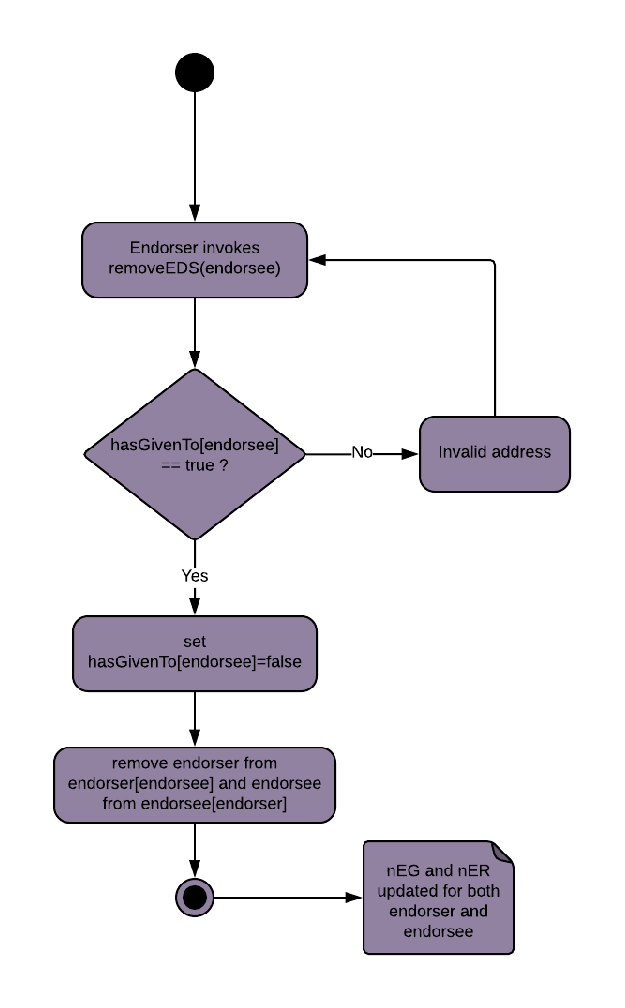
\includegraphics[width=0.5\textwidth]{Images/ActivityDiagramRemoveEDS.eps}
	\caption{Activity diagram for removing endorsement}
	\label{fig:removeEds}
\end{figure}

\subsection{SmartContract} 
Smart contracts can be either deterministic which doesn't require any
information from outside blockchain or non-deterministic which does need to get
oracles from external sources\cite{alharby2017blockchain}. For this PoC,
endorsement contract is deterministic and so all the data and variables
required are stored and executed on the blockchain. \\
Figure ~\ref{fig:smartcontracts}, represents the system of smart contracts as a
way to visualize the component layer and is based on \cite{delmolino2016step}. 
The main contracts written for this PoC are : 
\begin{itemize}
	\item Ownable: tracks the owner of the contract. i.e., the creator of
		contract. 
	\item killable: inherits from ownable and can be killed by owner only. 
	\item Participants: set participant and store their information. An index
		to access each participant. 
	\item Endorsement: It inherits from participants and can be called by
		participants only. Endorsement contract handles the core logic of
		endorsement system, accesses/queries addresses from Participants and is
		used for storage of data along with CRUD operations on them.  
	\item Computation: inherits from Endorsement contract and allows anyone to
		get the final score by accessing the current state from an Endorsement
		contract.
	\item Marketplace: stores the buyers, sellers information and allows them
		to buy or sell the product. Also, allows buyer/seller to compute the
		score of the involved entity before doing a transaction.  
\end{itemize}

'Marketplace' contract was written to test the endorsement network on a
transactional network. However, when deploying endorsement system in the real
world, other transactional network/online systems are assumed to have their
reputation platform. The reputation platform should have assigned a score to
the corresponding users based on the behavior on that network. The endorsement
system can act as additional conformity for deciding on a transaction. Say,
Alice is registered on Endorsement network and has made a decent score. If she
wants to sell a product on Marketplace(or any other transactional network), she
can claim about her score and anyone who wants to buy from Alice can verify the
claim by checking the score that corresponds to her public address. If both
Alice and buyer are registered on the endorsement network on the blockchain,
they can send a pre-transaction message to each other to verify that Alice is
who she claims to be and vice-versa. In case the buyer is not registered on the
endorsement network then Alice can prove the claim by signing a cryptographic
challenge with her private key. 

\begin{figure}
	\centering
	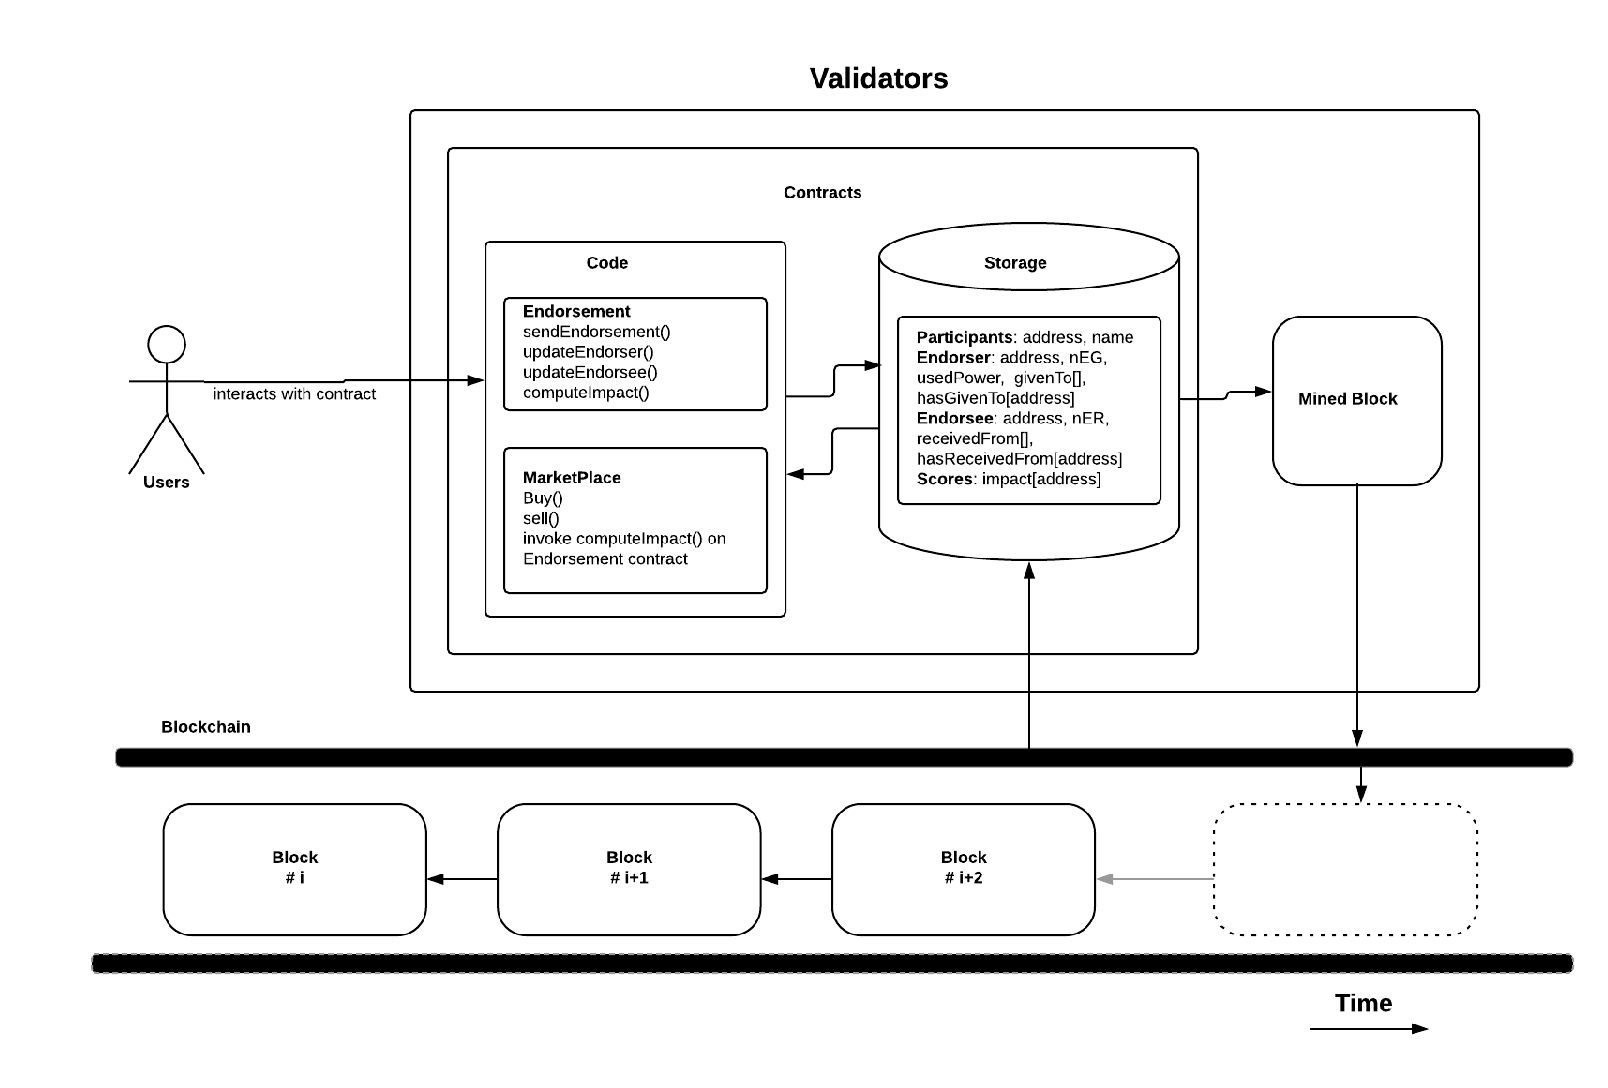
\includegraphics[width=1.0\textwidth]{Images/SmartContractsEDSMarketPlace.eps}
	\caption{Smart contract system}
	\label{fig:smartcontracts}
\end{figure}


\subsection{Data and variables on and off blockchain}
For this PoC, the data required to identify the users are stored on the
blockchain. But, it does preserve the anonymity requirement mentioned in
section ~\ref{ch:UserStories}, as the only public information is the link
between the public key hash and individual trust score. Even though the users
are required to register with a pseudonym, it is not needed that the aliases be
linked to real-world identity. A user might like to share more
information(other online account ids, address, etc.).  As mentioned earlier in
the gas consumption section, every non-zero byte data or code of a transaction
costs a certain amount of gas \cite{buterin2013ethereum}. Storing this data can
become an expensive operation for real-world usage. The right approach can be
to use an off-blockchain storage solution such as IPFS, swarm
\cite{benet2014ipfs}. The hash that points to the file in IPFS can then be
stored on the blockchain.  Generally, client-side assets (HTML, js) are stored
on these distributed off-chain file system that can communicate to the
contracts registered on blockchain network. 

\subsection{Blockchain and Consensus algorithms}\label{subsec:bcConsensus}
The proposed platform for this PoC is Ethereum, continually developing open
source blockchain ecosystem. The process of starting up the nodes and deploying
the contract on the network is shown in figure ~\ref{fig:startup}. 
\begin{figure}
	\centering
	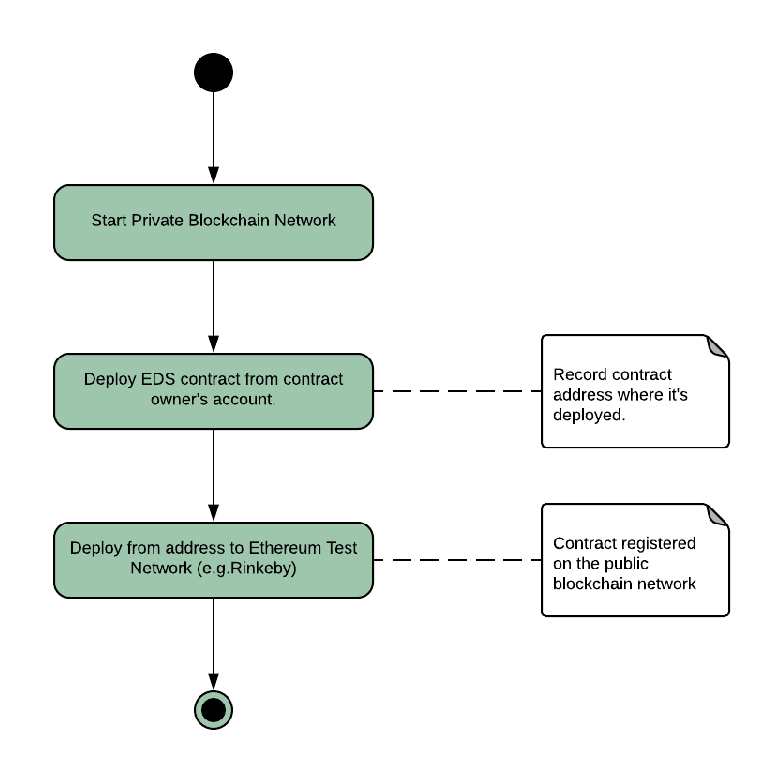
\includegraphics[width=0.6\textwidth]{Images/ActivityDiagramStartUpBC.eps}
	\caption{Startup activity for registering contract on the network}
	\label{fig:startup}
\end{figure}
As a permissionless system, it allows any nodes to collect transactions and act
as a writer. Consensus mechanism that is generally used in a permissionless
setting is Proof-of-Work or Proof-of-Stake. As mentioned earlier, PoW is
computationally expensive and wasteful. Using other consensus mechanisms such
as delegated proof of stake requires finding enough trustworthy validators that
can act as a leader or a master node which can be given authority to vote on
behalf of the community. In the endorsement network, an honest endorsement is
supposed to be between known entities. However, all participating entities do
not know each other, and no one node can be trusted to collect everyone's
transaction and make a final commit. Gochain \footnote{https://gochain.io/} has
mentioned the use of PoR(Proof-of-reputation) as a consensus mechanism in its
ethereum based blockchain platform. The basic idea here is to allow
participants on the network that have a high reputation to sign the block. It
builds on the theory that it is not worthwhile for a reputed node to tarnish
the current reputation that took some time and effort to create. The
endorsement system is designed to assign a global reputation score to each
entity and could use PoR. Since reputation scores are significant to maintain,
the nodes that have an impact score within some given range can be trusted to
validate and sign the blocks of transactions. PoR on endorsement system can
only be used if the endorsement that results in an impact value becomes a
valuable asset over time through extensive use. It is not recommended to start
with it. However, PoR can be used along with PoW from the beginning. As such,
the recommended consensus mechanism for the current design is PoW despite its
limitations. Various alternatives to PoW and consensus algorithms related
research that can solve specific problems(e.g., transaction speed, transaction
size, size of nodes, etc.) are under development. 
\begin{figure}[h]
	\centering
	\includegraphics[width=0.5\textwidth]{Images/ActivityDiagram.eps}
	\caption{Activity Diagram for sending an endorsement}
	\label{fig:activity}
\end{figure}
Hashgraph \cite{baird2016hashgraph}  proposes the recent advancement in
consensus engine that claims to be fair, fast and Byzantine fault tolerant. It
is based on gossip protocol(nodes gossip about transactions and gossip) and
offers mathematical proof on the total order of transactions with less
communication overhead. However, the hashgraph conundrum is that their software
is patented unlike other developments in the similar space. A developer must
pay for making an API call using micropayment of the platform.  Endorsement
system can also be used on a permissioned setting, much like sovrin
\cite{tobin2016inevitable} does.  Sovrin introduces a steward node who is
trusted based on a signed agreement with sovrin
\footnote{https://sovrin.org/library/steward-agreement/} and has received
approval as trusted institutions. The concept of steward nodes might be
questionable regarding full decentralization, but there are cases when this
level of decentralization is enough for the security of an application.   For
instance, there can be a consortium of e-commerce organizations that could
agree on a specific set of protocols. Validation of transactions can be based
on a voting mechanism that requires the consent of 2/3 of the trusted members.
Doing so can increase the transaction validation time compared to PoW.   

\subsection{Graph based algorithm for anomaly detection}

%\section{Honest vs. Malicious Nodes}

%User profile : 
% consistent
% declining reputation
% progressing reputation

% The idea is not to exclude malicious behavior in the network, rather include them 
% but give them no value. The endorsement power diminishes every time an entity 
% gives it to someone so the right thing to do for any entity would be to use 
% them wisely. 
% It can be analogous to a gameplay where a player is not restricted to 
% drink a life potion when his lifebar is full but he will waste it if he does with 
% no impact and when the time comes to use it, there won't be any more potion left. 


% drinking potion when you have full life 

%consensus algorithm - 
%what stops someone from making 250 nodes and just endorsing 
%themself.  - net flow rate convergence ,
% would detect this. as we can all 250 nodes are created just to endorse this one 
% node, and so those nodes value would soon converge to zero. 
 
 
%  Problem: What happens if someone plays well in the network for a long time and in 
%  the end decides to betray the whole network. (spy)


% The goal is : once a dishonest node is detected by reputation algorithm in a 
% transaction network, all their endorsement given or received is automatically removed 
% from the network so that will change the values in the dishonest node and other nodes 
% that were connected to it in the past. 

% net flow rate convergence can also be used to determine anomaly in the network. 

% incentivize honest behaviour.


%Model as interaction graph
%quantify endorsement as reputation score and translate to trust value
%mention reputation algorithm as necessary to be used on the n/w. 

%\section{Trust Metrics}

%central nodes, 
%How is trust measured?
%What is required for it to be a correct solution? 
%objective way of accepting or rejecting the work
%Every node keeps track of its neighbouring node and whenever an intera



%\section{Experimental Setup} \label{sec:sectionlabel}

%Test Network describe, no. of nodes, level of difficulty etc.

%\section{second section}
% It may include: Description of the methodological, theoretical, conceptual or empirical framework; design of the
% experiment; relevant steps of reasoning; data description and sources.

% Describe the approach and method(s) used to address the scientific problem. Also reflect on the particular choice of method and justify it.
